%%%%%%%%%%%%%%%%%%%%%%%%%%%%%%%%%%%%%%%%% 
% Beamer Presentation
% LaTeX Template
% Version 1.0 (10/11/12)
% 
% This template has been downloaded from:
% http://www.LaTeXTemplates.com
% 
% License:
% CC BY-NC-SA 3.0 (http://creativecommons.org/licenses/by-nc-sa/3.0/)
% 
%%%%%%%%%%%%%%%%%%%%%%%%%%%%%%%%%%%%%%%%% 

% ----------------------------------------------------------------------------------------
%	PACKAGES AND THEMES
% ----------------------------------------------------------------------------------------

\documentclass{beamer}

\mode<presentation> {

  % The Beamer class comes with a number of default slide themes
  % which change the colors and layouts of slides. Below this is a list
  % of all the themes, uncomment each in turn to see what they look like.

  % \usetheme{default}
  % \usetheme{AnnArbor}
  % \usetheme{Antibes}
  % \usetheme{Bergen}
  % \usetheme{Berkeley}
  % \usetheme{Berlin}
  % \usetheme{Boadilla}
  % \usetheme{CambridgeUS}
  % \usetheme{Copenhagen}
  % \usetheme{Darmstadt}
  % \usetheme{Dresden}
  % \usetheme{Frankfurt}
  % \usetheme{Goettingen}
  % \usetheme{Hannover}
  % \usetheme{Ilmenau}
  % \usetheme{JuanLesPins}
  % \usetheme{Luebeck}
  \usetheme{Madrid}
  % \usetheme{Malmoe}
  % \usetheme{Marburg}
  % \usetheme{Montpellier}
  % \usetheme{PaloAlto}
  % \usetheme{Pittsburgh}
  % \usetheme{Rochester}
  % \usetheme{Singapore}
  % \usetheme{Szeged}
  % \usetheme{Warsaw}

  % As well as themes, the Beamer class has a number of color themes
  % for any slide theme. Uncomment each of these in turn to see how it
  % changes the colors of your current slide theme.

  % \usecolortheme{albatross}
  % \usecolortheme{beaver}
  % \usecolortheme{beetle}
  % \usecolortheme{crane}
  % \usecolortheme{dolphin}
  % \usecolortheme{dove}
  % \usecolortheme{fly}
  % \usecolortheme{lily}
  % \usecolortheme{orchid}
  % \usecolortheme{rose}
  % \usecolortheme{seagull}
  % \usecolortheme{seahorse}
  % \usecolortheme{whale}
  % \usecolortheme{wolverine}

  % \setbeamertemplate{footline} % To remove the footer line in all slides uncomment this line
  % \setbeamertemplate{footline}[page number] % To replace the footer line in all slides with a simple slide count uncomment this line

  % \setbeamertemplate{navigation symbols}{} % To remove the navigation symbols from the bottom of all slides uncomment this line
}

\usepackage{graphicx} % Allows including images
\usepackage{multirow}
\usepackage{booktabs} % Allows the use of \toprule, \midrule and \bottomrule in tables
\graphicspath{ {images/} }

% ----------------------------------------------------------------------------------------
%	TITLE PAGE
% ----------------------------------------------------------------------------------------

\title[Powered by Python]{Regression Flow Introduction} % The short title appears at the bottom of every slide, the full title is only on the title page

\author{Guanyu Yi} % Your name
\institute[SPRD] % Your institution as it will appear on the bottom of every slide, may be shorthand to save space
{
  Spreadtrum Communications, Inc. \\ % Your institution for the title page
  \medskip
  \textit{guanyu.yi@spreadtrum.com} % Your email address
}
\date{July 23, 2015} % Date, can be changed to a custom date

\begin{document}

\begin{frame}
  \titlepage % Print the title page as the first slide
\end{frame}

\begin{frame}
  \frametitle{Overview} % Table of contents slide, comment this block out to remove it
  \tableofcontents % Throughout your presentation, if you choose to use \section{} and \subsection{} commands, these will automatically be printed on this slide as an overview of your presentation
\end{frame}

% ----------------------------------------------------------------------------------------
%	PRESENTATION SLIDES
% ----------------------------------------------------------------------------------------

% ------------------------------------------------
\section{SPRD Regression} % Sections can be created in order to organize your presentation into discrete blocks, all sections and subsections are automatically printed in the table of contents as an overview of the talk
% ------------------------------------------------

\begin{frame}
  \frametitle{SPRD Regression}
  \begin{itemize}
  \item python3 \texttt{+} database \texttt{+} server \texttt{+} dynamic webpages
  \item used in projects such as Whale, Whale2, LTEA\_TC etc.
  \item concurrent architecture
  \item extensible platform
  \item unique accessing address for all sites in UNIX net \textbf{http://shvp01:8000}
  \item easy to maintain and update
  \end{itemize}
\end{frame}

% ------------------------------------------------
\section{Platform Overview}
% ------------------------------------------------

\begin{frame}
  \frametitle{Platform Overview}
  \begin{figure}
    \centering
    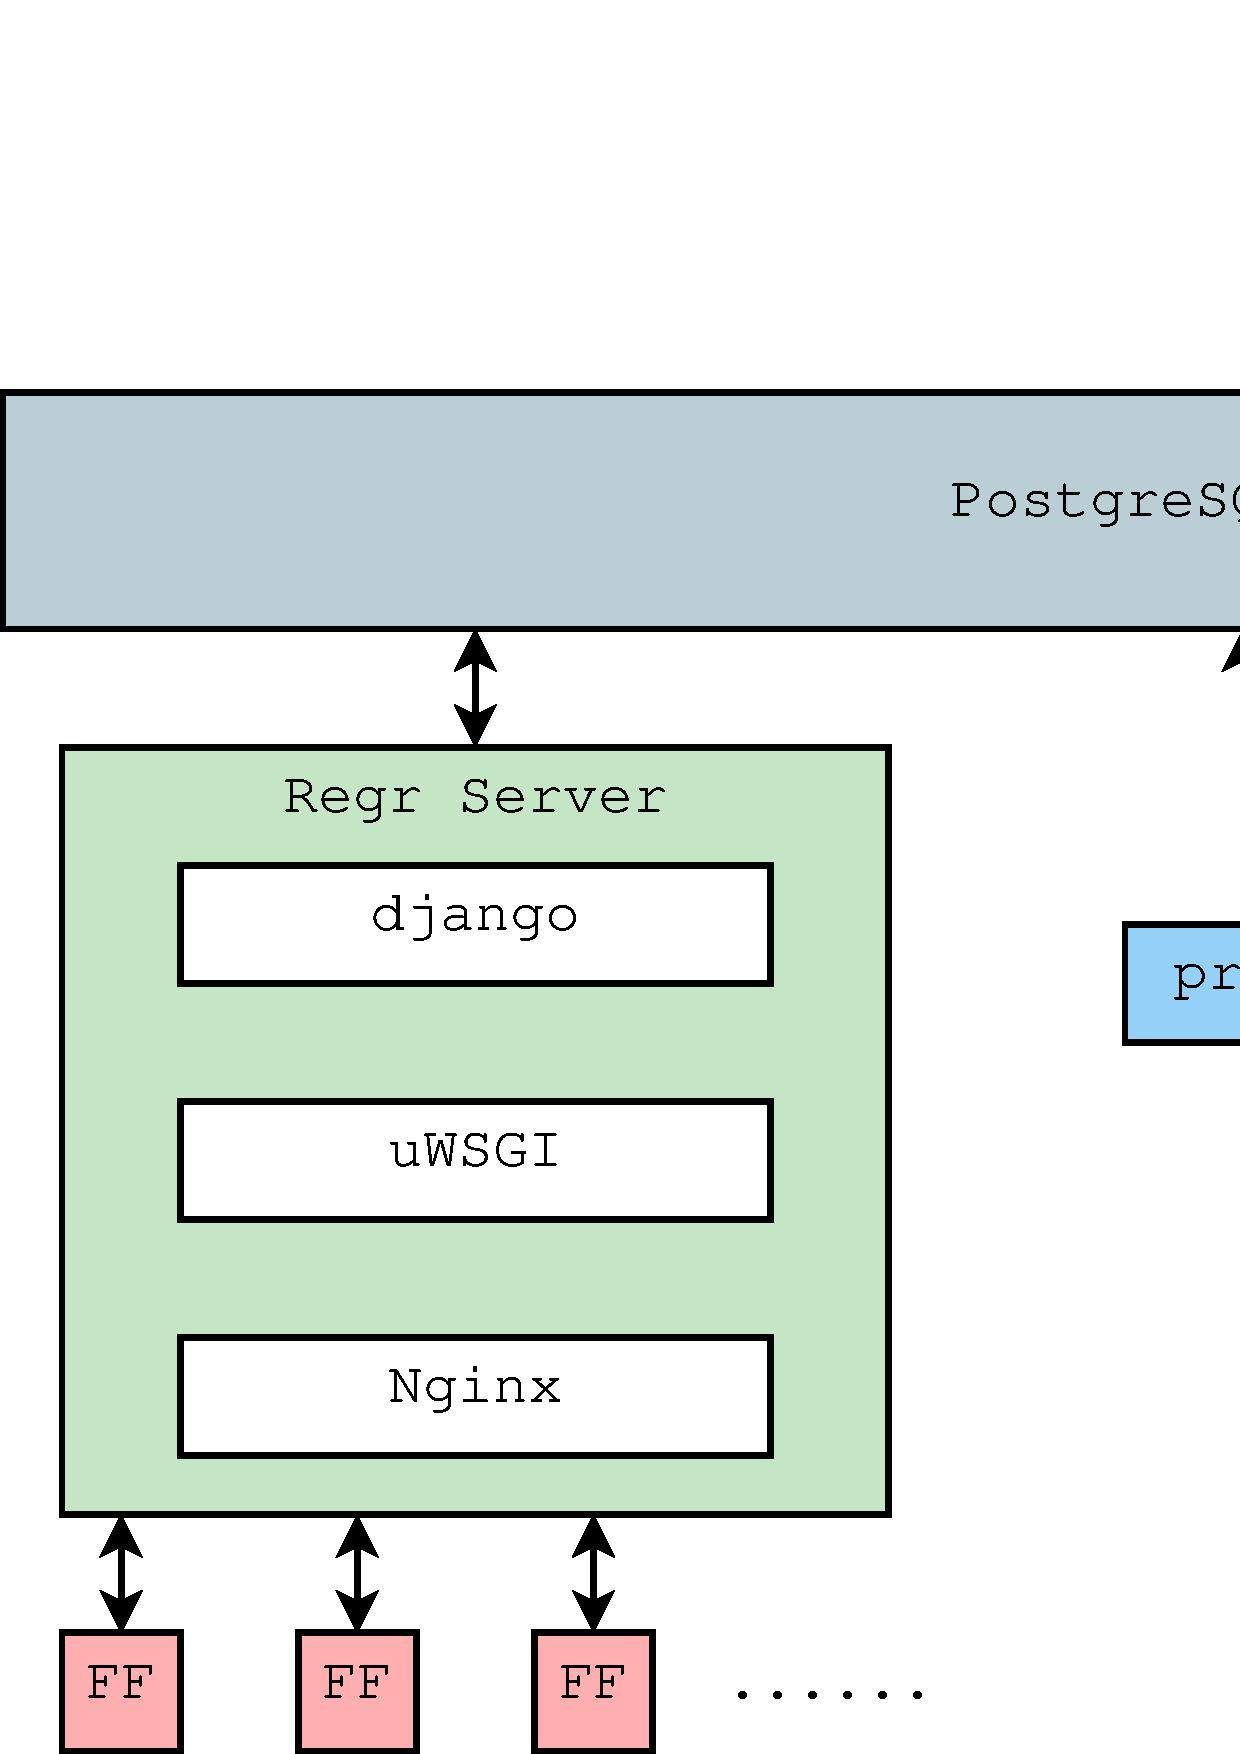
\includegraphics[width=0.9\linewidth]{regr_struc}
    \caption{Regression platform structure}
  \end{figure}
\end{frame}

% ------------------------------------------------
\section{Flow and Commands}
% ------------------------------------------------

\begin{frame}
  \frametitle{Flow and Commands}
  \begin{block}{Kicking off regression}
    \begin{itemize}
    \item \textbf{prun regr -f TRACELISTS} to kick off all test cases of tracelists in parallel (.ini, .cfg, .xls, .xlsx)
    \item other options...
    \end{itemize}
  \end{block}

  \begin{block}{Submitting LSF jobs}
    \begin{itemize}
    \item invoking runsim.pl
    \item submitting jobs into LSF cluster in parallel
    \end{itemize}
  \end{block}

  \begin{block}{Checking regression reports}
    \begin{itemize}
    \item accessing to regression server \textbf{http://shvp01:8000/regr}
    \item useful alias \textbf{rrpt REPORTER\_NAME}
    \item remove $\sim$/.mozilla if using the alias for the first time
    \end{itemize}
  \end{block}
\end{frame}

% ----------------------------------------------------------------------------------------

\begin{frame}
  \frametitle{Flow and Commands}
  \begin{block}{Full mode}
    \begin{itemize}
    \item kicking off cases no matter what the previous results are
    \item default mode
    \item usually used in mini set regression or the regression after a long term
    \end{itemize}
  \end{block}

  \begin{block}{Failed mode}
    \begin{itemize}
    \item kicking off only the cases failed in the last round of regression
    \item option \textbf{-fm}
    \item usually used in recursive regression kicking off to save LSF resources
    \end{itemize}
  \end{block}

  \begin{block}{Options}
    \begin{itemize}
    \item LSF specifications, kicking off particular cases, etc.
    \item refer to \textbf{prun regr -h} for more interesting options...
    \end{itemize}
  \end{block}
\end{frame}

% ----------------------------------------------------------------------------------------

\begin{frame}
  \frametitle{Flow and Commands}
  \begin{block}{Coverage generation}
    \begin{itemize}
    \item adding \textbf{-cov} option when kicking off regression
    \item \textbf{prun merge -p} to generate a full DUT coverage database as base
    \item \textbf{prun merge -d MERGE\_DIRS} to generate subsys merged coverage database in parallel, and then to merge all coverage database together based on the base database
    \item \textbf{prun merge -r} to generate entire structural html based coverage report
    \end{itemize}
  \end{block}

  \begin{block}{Options}
    \begin{itemize}
    \item LSF specifications, vrefine file, etc.
    \item refer to \textbf{prun merge -h} for more options...
    \end{itemize}
  \end{block}
\end{frame}

% ------------------------------------------------
\section{Directory Hierarchy}
% ------------------------------------------------

\begin{frame}
  \frametitle{Directory Hierarchy}
  \begin{columns}[c] % The "c" option specifies centered vertical alignment while the "t" option is used for top vertical alignment

    \column{.45\textwidth} % Left column and width
    \begin{figure}
      \centering
      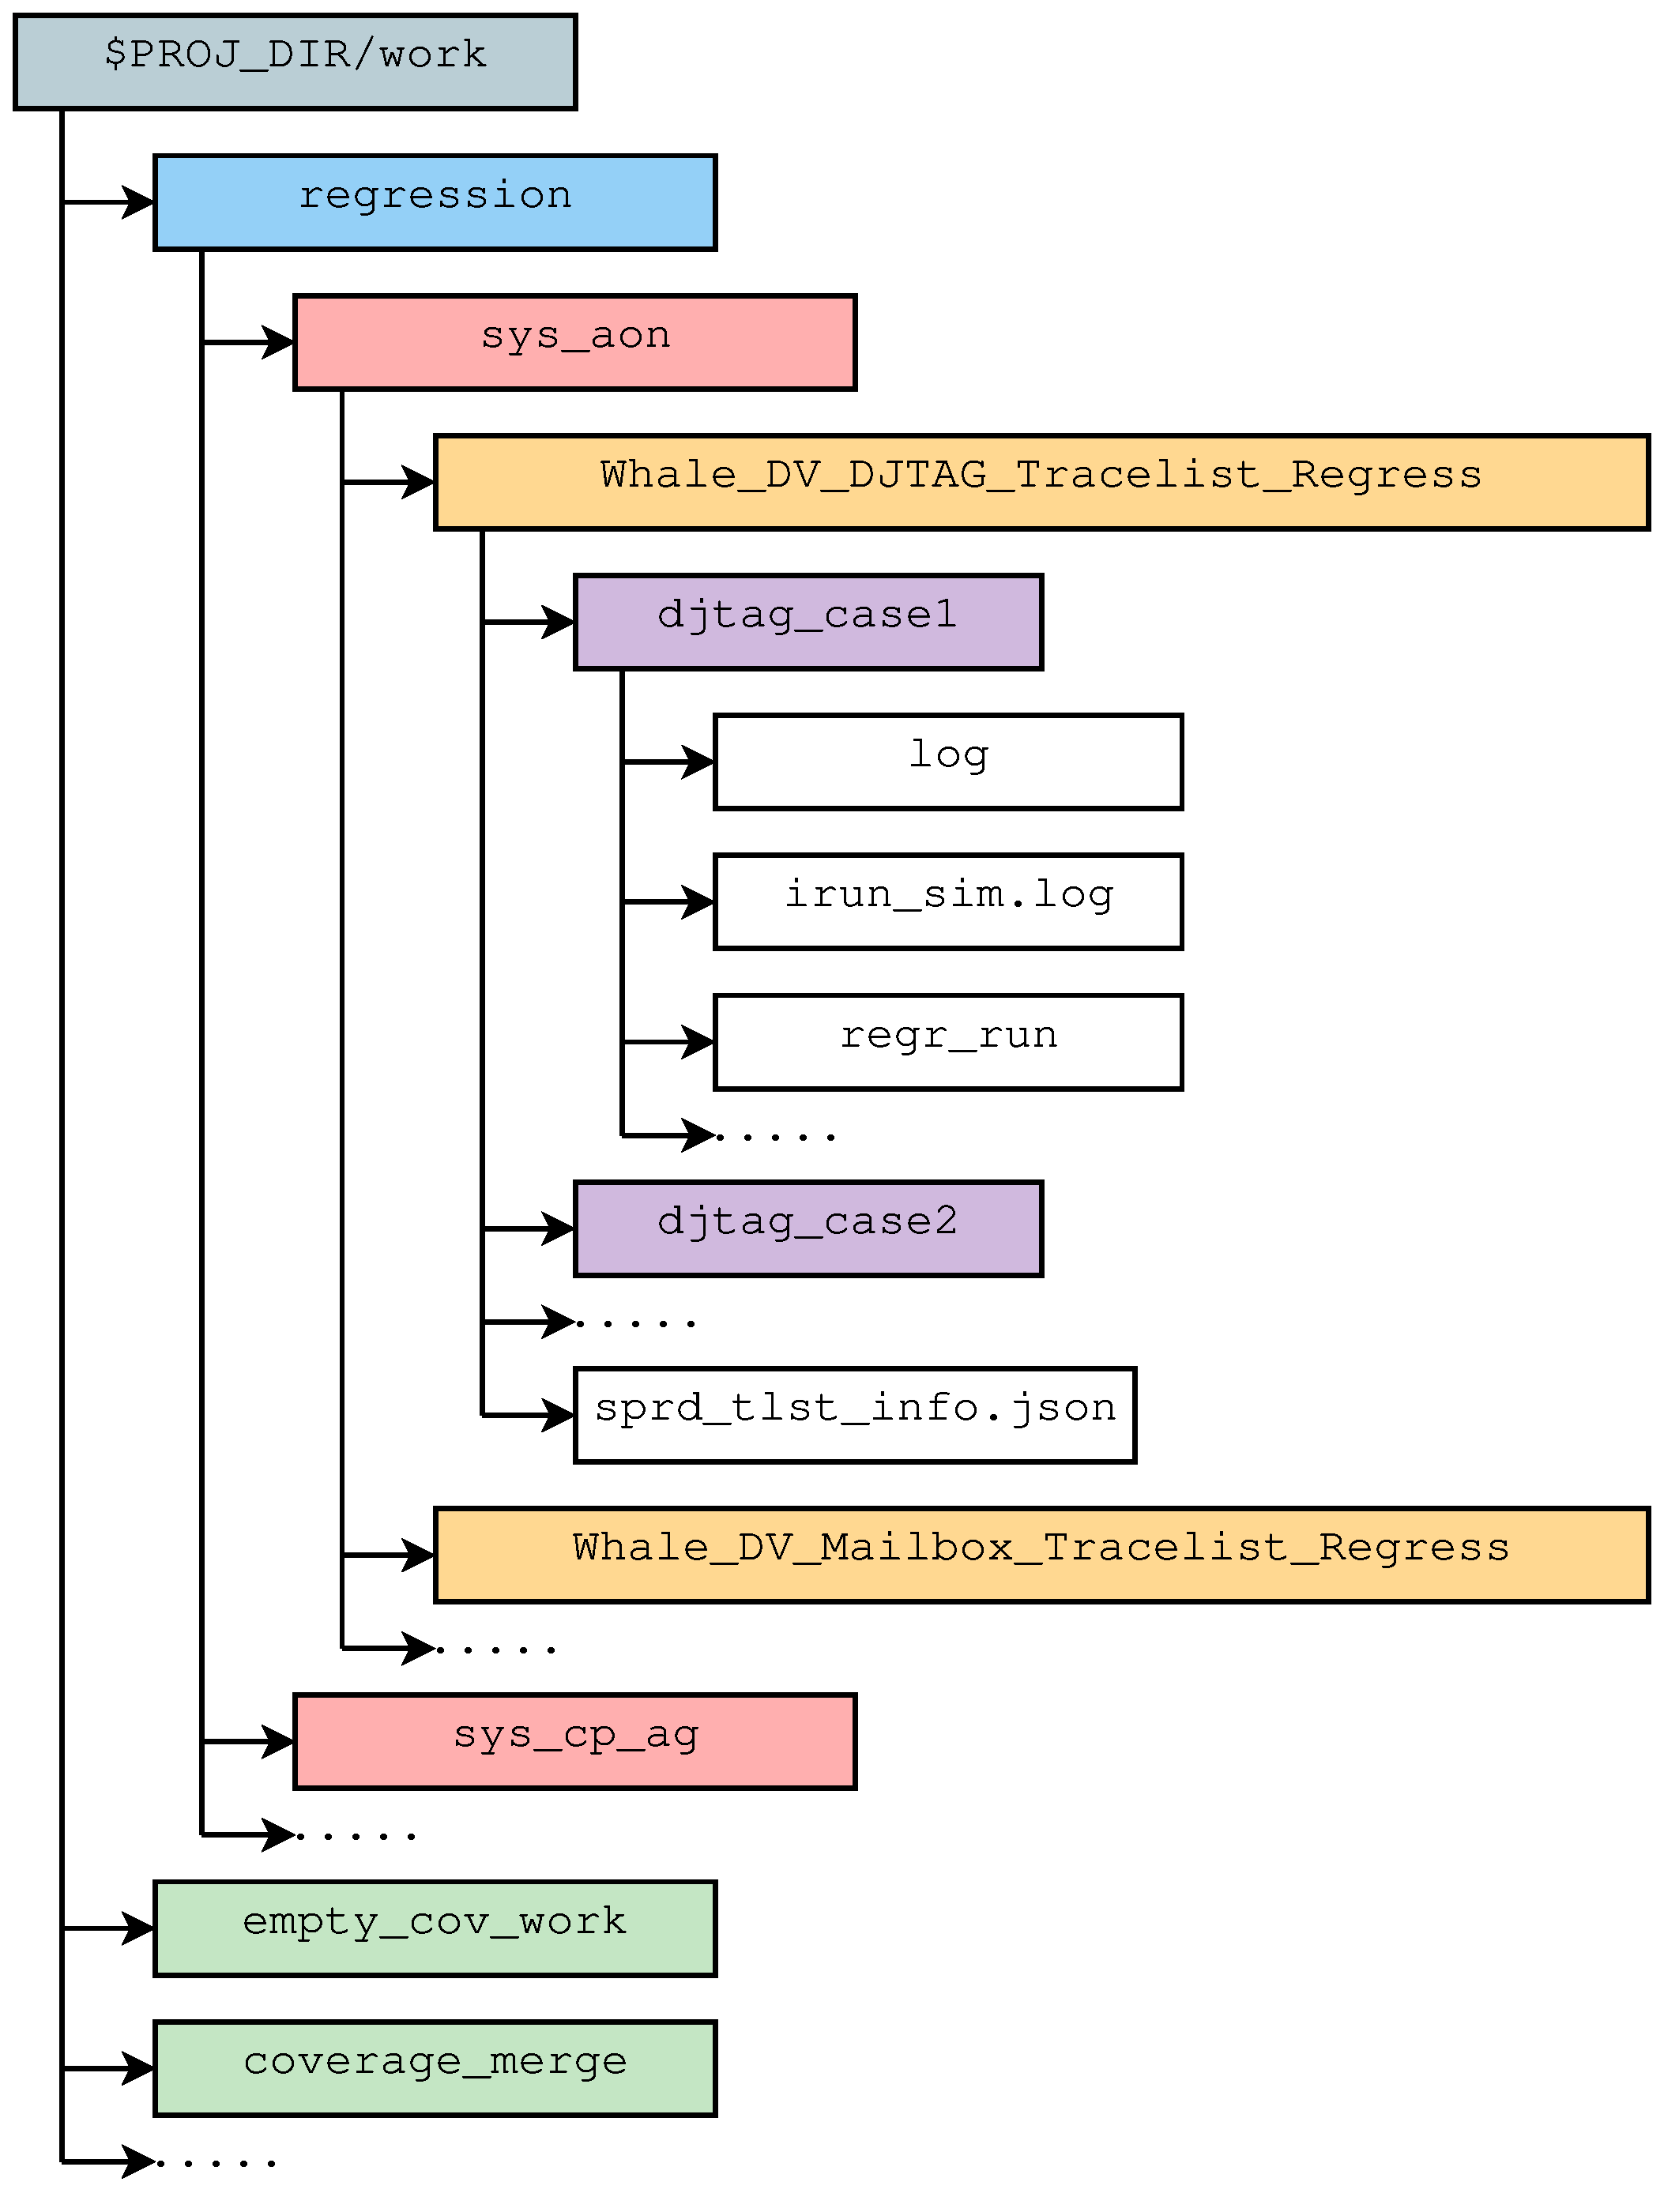
\includegraphics[width=0.9\linewidth]{dir_regr_hier}
      \caption{Regression directory}
    \end{figure}

    \column{.5\textwidth} % Right column and width
    \begin{figure}
      \centering
      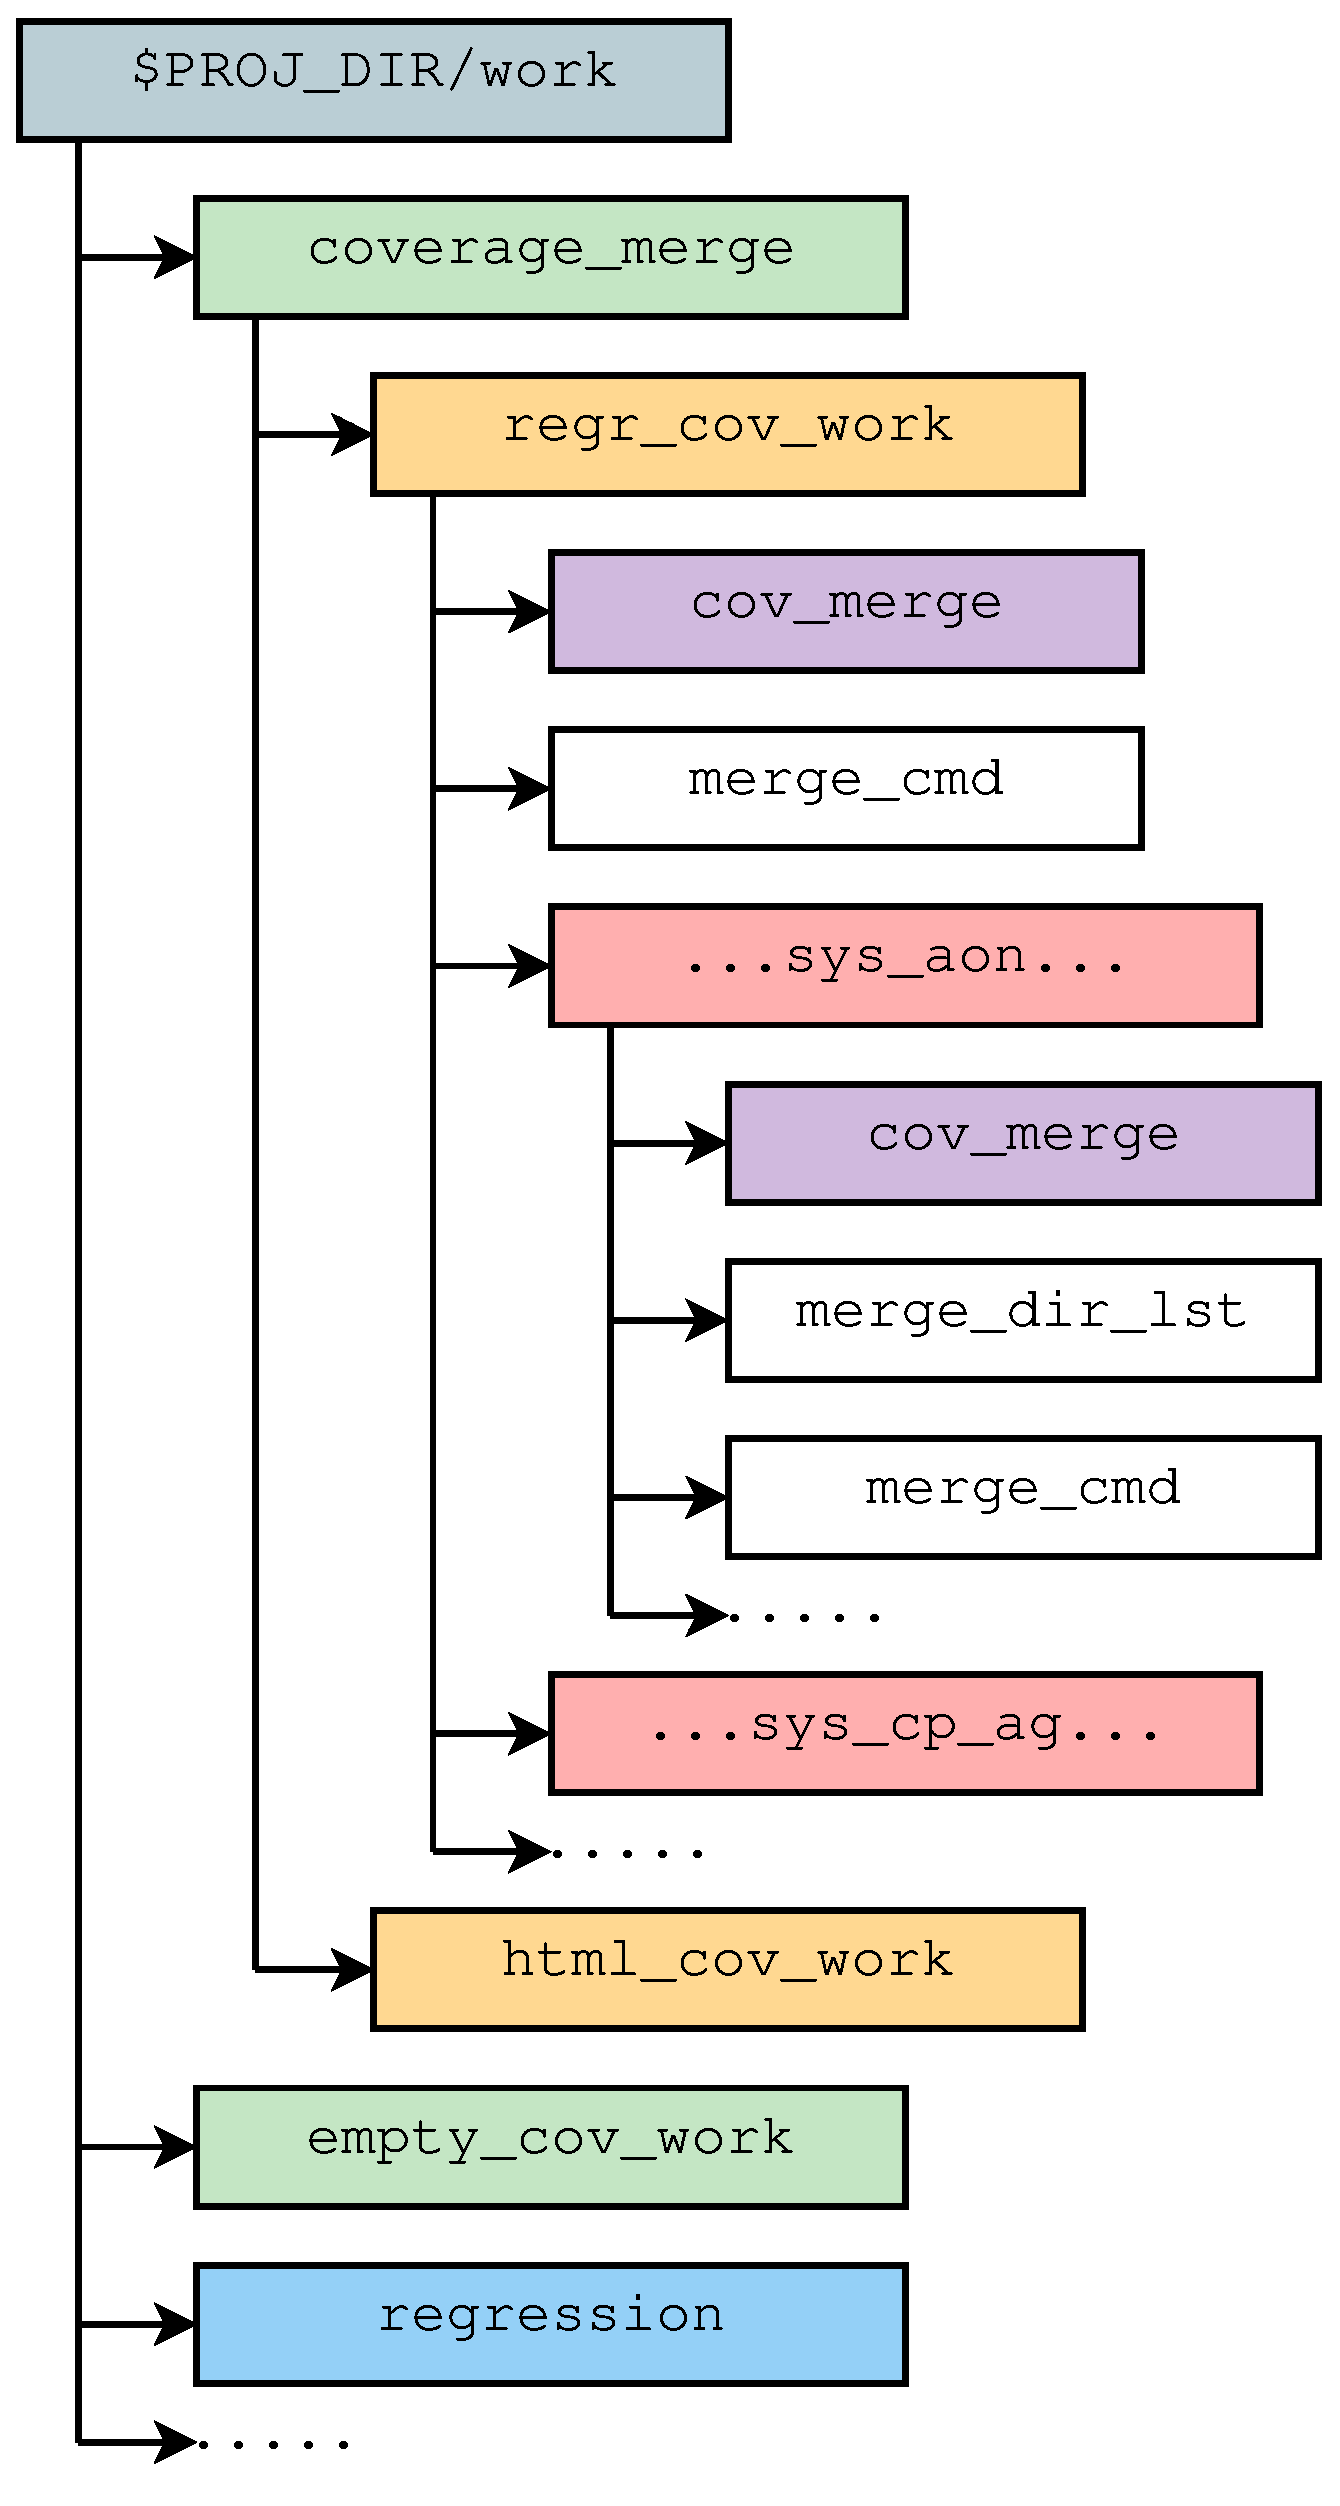
\includegraphics[width=0.57\linewidth]{dir_cov_hier}
      \caption{Coverage directory}
    \end{figure}

  \end{columns}
\end{frame}

% ------------------------------------------------
\section{Tracelist File Format}
% ------------------------------------------------

\begin{frame}
  \frametitle{Tracelist File Format}
  \begin{itemize}
  \item Supported tracelist format: .xls, .xlsx, .ini, .cfg
  \item templates location: \$PROJ\_DIR/env/tracelist
  \item \textbf{prun regr -c TRACELIST} to check tracelist format
  \item \textbf{prun regr -c -ini TRACELIST} to convert excel to unix config
  \end{itemize}
\end{frame}

% ----------------------------------------------------------------------------------------

\begin{frame}
  \frametitle{Tracelist File Format}
  \textbf{Home}
  \begin{itemize}
  \item fill in the blanks according to the topic
  \item script directory should be the directory where your customized script located; omitted if only runsim.pl is used
  \end{itemize}

  \begin{figure}
    \centering
    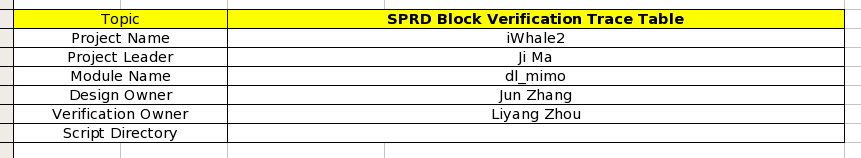
\includegraphics[width=0.9\linewidth]{home_sheet}
    \caption{Regression tracelist Home sheet}
  \end{figure}
\end{frame}

% ----------------------------------------------------------------------------------------

\begin{frame}
  \frametitle{Tracelist File Format}
  \textbf{Testcase Plan}
  \begin{itemize}
  \item case\_name, sim\_type, simulation\_command in one row
  \item multiple sim\_types split by comma(\textbf{,})
  \item case\_name must be unique
  \item each case must have one type of rtl0.1, rtl0.5 and rtl0.9
  \end{itemize}

  \begin{figure}
    \centering
    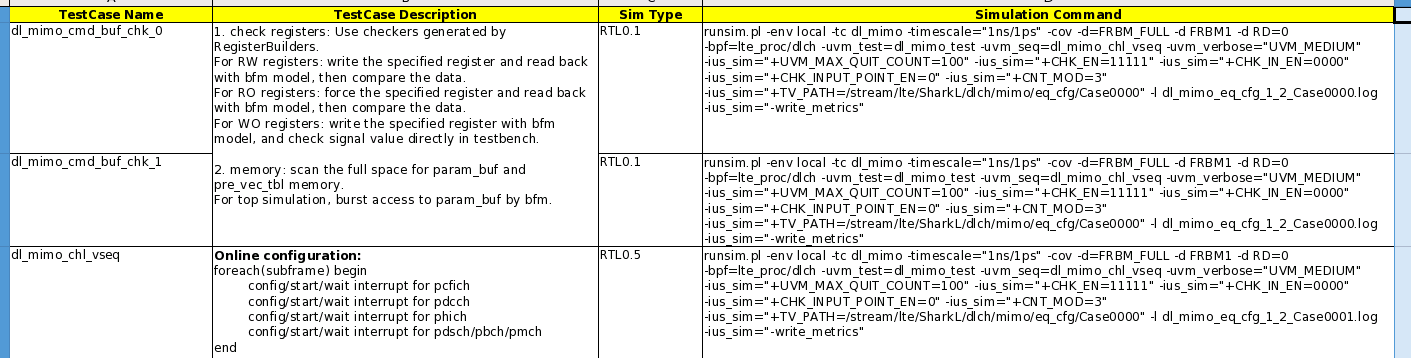
\includegraphics[width=\linewidth]{tp_sheet}
    \caption{Regression tracelist Testcase Plan sheet}
  \end{figure}
\end{frame}

% ----------------------------------------------------------------------------------------

\begin{frame}
  \frametitle{Tracelist File Format}
  \begin{table}
    \begin{tabular}{ll}
      \toprule
      \textbf{Sim Type} & \textbf{Description}\\
      \midrule
      RTL0.1 & Case set to meet RTL0.1 requirement\\
      RTL0.5 & Case set to meet RTL0.5 requirement\\
      RTL0.9 & Case set to meet RTL0.9 requirement\\
      DV\_POWER & Power simulation case set\\
      DV\_POST & Post simulation case set\\
      DV\_MAN & Manually checked case set\\
      DV\_LOCAL & Local cases for IP\\
      \bottomrule
    \end{tabular}
    \caption{Regression Sim Type table}
  \end{table}
\end{frame}

% ----------------------------------------------------------------------------------------

\begin{frame}
  \frametitle{Tracelist File Format}
  \textbf{Regression Configuration}
  \begin{itemize}
  \item customized no check string has highest priority to ignore the corresponding lines
  \item customized error string has middle priority to trigger status to error
  \item customized pass string has lowest priority to trigger status to pass
  \item it is better to leave them blank if you don't know what they are
  \end{itemize}

  \begin{figure}
    \centering
    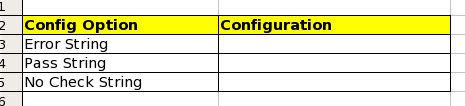
\includegraphics[width=0.5\linewidth]{rc_sheet}
    \caption{Regression tracelist Regression Configuration sheet}
  \end{figure}
\end{frame}

% ----------------------------------------------------------------------------------------

\begin{frame}
  \frametitle{Tracelist File Format}
  \textbf{UNIX config tracelist format}
  \begin{itemize}
  \item text format
  \item easy to update and diff using editors and version control system
  \item fewer tracelist format issues
  \end{itemize}
\end{frame}

% ------------------------------------------------
\section{prun API}
% ------------------------------------------------

\begin{frame}
  \frametitle{prun API}
  \begin{figure}
    \centering
    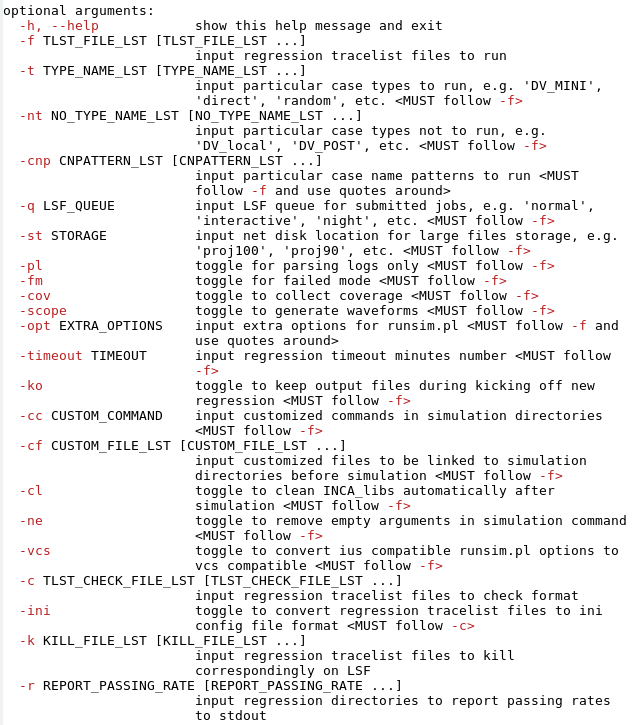
\includegraphics[width=0.54\linewidth]{prun_api}
  \end{figure}
\end{frame}

% ----------------------------------------------------------------------------------------

\begin{frame}
  \Huge{\centerline{Q \& A}}
\end{frame}

% ----------------------------------------------------------------------------------------

\end{document} 
%%% Local Variables:
%%% mode: latex
%%% TeX-master: t
%%% End:
